% Copyright (C) 2014-2016 by Thomas Auzinger <thomas@auzinger.name>

\documentclass[draft,final]{vutinfth} % Remove option 'final' to obtain debug information.

% Load packages to allow in- and output of non-ASCII characters.
\usepackage{lmodern}        % Use an extension of the original Computer Modern font to minimize the use of bitmapped letters.
\usepackage[T1]{fontenc}    % Determines font encoding of the output. Font packages have to be included before this line.
\usepackage[utf8]{inputenc} % Determines encoding of the input. All input files have to use UTF8 encoding.

% Extended LaTeX functionality is enables by including packages with \usepackage{...}.
\usepackage{amsmath}    % Extended typesetting of mathematical expression.
\usepackage{amssymb}    % Provides a multitude of mathematical symbols.
\usepackage{mathtools}  % Further extensions of mathematical typesetting.
\usepackage{microtype}  % Small-scale typographic enhancements.
\usepackage[inline]{enumitem} % User control over the layout of lists (itemize, enumerate, description).
\usepackage{multirow}   % Allows table elements to span several rows.
\usepackage{booktabs}   % Improves the typesettings of tables.
\usepackage{subcaption} % Allows the use of subfigures and enables their referencing.
\usepackage[ruled,linesnumbered,algochapter]{algorithm2e} % Enables the writing of pseudo code.
\usepackage[usenames,dvipsnames,table]{xcolor} % Allows the definition and use of colors. This package has to be included before tikz.
\usepackage{nag}       % Issues warnings when best practices in writing LaTeX documents are violated.
\usepackage{todonotes} % Provides tooltip-like todo notes.

\usepackage{menukeys}

% fnurl adapted from http://tex.stackexchange.com/questions/115479/insert-footnotes-with-href
\usepackage{hyperref}  % Enables cross linking in the electronic document version. This package has to be included second to last.
\newcommand\fnurl[2]{%
  \href{#1}{#2}\footnote{\url{#1}}%
}

\usepackage[acronym,toc]{glossaries} % Enables the generation of glossaries and lists fo acronyms. This package has to be included last.

% Define convenience functions to use the author name and the thesis title in the PDF document properties.
\newcommand{\authorname}{Kevin Singer} % The author name without titles.
\newcommand{\thesistitle}{Title of the Thesis} % TODO The title of the thesis. The English version should be used, if it exists.
% TODO
% * a study
% * architectur
% * includes tooling
% * client side app

% Set PDF document properties
\hypersetup{
    pdfpagelayout   = TwoPageRight,           % How the document is shown in PDF viewers (optional).
    linkbordercolor = {Melon},                % The color of the borders of boxes around crosslinks (optional).
    pdfauthor       = {\authorname},          % The author's name in the document properties (optional).
    pdftitle        = {\thesistitle},         % The document's title in the document properties (optional).
    pdfsubject      = {Subject},              % The document's subject in the document properties (optional).
    pdfkeywords     = {a, list, of, keywords} % The document's keywords in the document properties (optional).
}

\setpnumwidth{2.5em}        % Avoid overfull hboxes in the table of contents (see memoir manual).
\setsecnumdepth{subsection} % Enumerate subsections.

\nonzeroparskip             % Create space between paragraphs (optional).
\setlength{\parindent}{0pt} % Remove paragraph identation (optional).

\makeindex      % Use an optional index.
\makeglossaries % Use an optional glossary.
%\glstocfalse   % Remove the glossaries from the table of contents.

% Set persons with 4 arguments:
%  {title before name}{name}{title after name}{gender}
%  where both titles are optional (i.e. can be given as empty brackets {}).
\setauthor{Pretitle}{\authorname}{Posttitle}{female}
\setadvisor{Pretitle}{Forename Surname}{Posttitle}{male}

% For bachelor and master theses:
\setfirstassistant{Pretitle}{Forename Surname}{Posttitle}{male}
\setsecondassistant{Pretitle}{Forename Surname}{Posttitle}{male}
\setthirdassistant{Pretitle}{Forename Surname}{Posttitle}{male}

% For dissertations:
\setfirstreviewer{Pretitle}{Forename Surname}{Posttitle}{male}
\setsecondreviewer{Pretitle}{Forename Surname}{Posttitle}{male}

% For dissertations at the PhD School and optionally for dissertations:
\setsecondadvisor{Pretitle}{Forename Surname}{Posttitle}{male} % Comment to remove.

% Required data.
\setaddress{Address}
\setregnumber{0123456}
\setdate{01}{01}{2001} % Set date with 3 arguments: {day}{month}{year}.
\settitle{\thesistitle}{Titel der Arbeit} % Sets English and German version of the title (both can be English or German).
\setsubtitle{Optional Subtitle of the Thesis}{Optionaler Untertitel der Arbeit} % Sets English and German version of the subtitle (both can be English or German).

% Select the thesis type: bachelor / master / doctor / phd-school.
% Bachelor:
\setthesis{bachelor}
%
% Master:
%\setthesis{master}
%\setmasterdegree{dipl.} % dipl. / rer.nat. / rer.soc.oec. / master
%
% Doctor:
%\setthesis{doctor}
%\setdoctordegree{rer.soc.oec.}% rer.nat. / techn. / rer.soc.oec.
%
% Doctor at the PhD School
%\setthesis{phd-school} % Deactivate non-English title pages (see below)

% For bachelor and master:
\setcurriculum{Media Informatics and Visual Computing}{Medieninformatik und Visual Computing} % Sets the English and German name of the curriculum.

% For dissertations at the PhD School:
\setfirstreviewerdata{Affiliation, Country}
\setsecondreviewerdata{Affiliation, Country}


\begin{document}

\frontmatter % Switches to roman numbering.
% The structure of the thesis has to conform to
%  http://www.informatik.tuwien.ac.at/dekanat

\addtitlepage{naustrian} % German title page (not for dissertations at the PhD School).
\addtitlepage{english} % English title page.
\addstatementpage

\begin{danksagung*}
\todo{Ihr Text hier.}
\end{danksagung*}

\begin{acknowledgements*}
\todo{Enter your text here.}
\end{acknowledgements*}

\begin{kurzfassung}
\todo{Ihr Text hier.}
\end{kurzfassung}

\begin{abstract}
\todo{Enter your text here.}
\end{abstract}

% Select the language of the thesis, e.g., english or naustrian.
\selectlanguage{english}

% Add a table of contents (toc).
\tableofcontents % Starred version, i.e., \tableofcontents*, removes the self-entry.

% Switch to arabic numbering and start the enumeration of chapters in the table of content.
\mainmatter

%\chapter{Introduction}
%\todo{Enter your text here.}

%\chapter{Additional Chapter}
%\todo{Enter your text here.}

% Remove following line for the final thesis.
%\input{intro.tex} % A short introduction to LaTeX.
\chapter{Introduction}

TODO -- abstract/introduction here %TODO

% use \begin{abstract}?

\chapter{Problem Description}\label{ref:probdescr}

This thesis is part of the over-arching project of crafting an
end-user-friendly
\fnurl{https://www.matchat.org/owner/}{client-application} for the
\fnurl{http://www.webofneeds.org/}{Web of Needs}
(\fnurl{http://sat.researchstudio.at/en/web-of-needs}{related
publications}), short WoN. The main focus was to research ways of
structuring the JavaScript-based client-application; thus it consisted
of researching and experimenting with state-of-the-art web-application
architectures and tooling, adapting and innovating on them for the
particular problem space, as well as identifying a migration path for
updating the existing code-base. To define the requirements, we first
need to take a high-level look over what the Web of Needs is and how
people can interact with it.

% problem-description\\
% * high-level\\
% * for people who aren't web-devs\\
% * pro problem ein satz: "prob ist im browser ld zu verwenden, dazu müssen sie geladen, geparst, gestored werden."\\

% Problemstellung (JS-Basisarchitektur für WoN-Owner App)\\
% as case study in architecture/migration\\

\todo{
define ontologies and rdf\\
\\
node = won-data/document-server\\
}


\section{Web of Needs}\label{web-of-needs}

It is a set of protocols (and reference implementations) that allow
posting documents, for instance describing supply and demand. Starkly
simplified examples would be ``I have a couch to give away'' or ``I'd
like to travel to Paris in a week and need transportation''. These
documents, called ``needs'' can be posted on arbitrary data servers
(called ``WoN-Nodes''). There they're discovered by matching-service,
that continuously crawls the nodes it finds. Additionally, to get faster
results, nodes can notify matchers of new needs. These then get compared
with the ones the matcher already knows about. If it finds a good pair
-- e.g. ``I have a couch to give away'' and ``Looking for furniture for
my living room'' -- the matcher notifies the owners of these needs. They
can then decide whether they want to contact each other. If they send
and accept each other's contact request, they can start chatting with
each other. The protocol in theory can also be used as a base-level for
other interactions, like entering into contracts or transferring money.

% PREVIOUSLY: It is a set of protocols (and reference implementations) that allow posting things like supply and demand (e.g. "I have a couch to give away") online on an arbitrary data server (called WoN-Node). These documents, called "needs", get discovered by a matching-service that notifies the owners of these needs (e.g. when the matcher finds someone that needs the couch offered). The protocols then allow for chatting (or other transactions) between the owners.

\section{Data on WoN-Nodes}\label{data-on-won-nodes}

Needs, connections between them and any events on those connections are
published on the WoN-Nodes in the form of RDF, which stands for
\fnurl{https://en.wikipedia.org/wiki/Resource_Description_Framework}{Resource
Description Framework}. In it, using a variety of different
syntax-alternatives, data is structured as a graph that can be
distributed over multiple (physical) resources. Edges in the graph in
their basic, most primitive form are described by triples of subject
(the start-node), predicates (the edge-type) and object (the
target-node). Note that subject and object need to be Unique Resource
Identifiers (URIs). Additionally, when using URIs, that also are Uniform
Resource Locators (URLs) -- together with the convention to publish data
for an RDF-node at that URL -- data-graphs on multiple servers can
easily be linked with each other, thus making them
\fnurl{https://en.wikipedia.org/wiki/Linked_data}{Linked Data}. This is a
necessary requirement for the Web of Needs, as data is naturally spread
out across several servers, i.e.~WoN-Nodes.

\begin{figure*}
\centering
\begin{verbatim}
<https://node.matchat.org/won/resource/need/7666110576054190000>
<http://purl.org/webofneeds/model#hasBasicNeedType>
<http://purl.org/webofneeds/model#Demand> .

<https://node.matchat.org/won/resource/need/7666110576054190000>
<http://purl.org/webofneeds/model#hasContent>
_:c14n0 .

<https://node.matchat.org/won/resource/need/7666110576054190000>
<http://www.w3.org/1999/02/22-rdf-syntax-ns#type>
<http://purl.org/webofneeds/model#Need> .

_:c14n0
<http://purl.org/dc/elements/1.1/title>
"Transportation Paris-Charles de Gaulle to City Center" .

_:c14n0
<http://purl.org/webofneeds/model#hasTextDescription>
"I’d like to travel to Paris in a week and need \
transportation (e.g. ride-sharing) from the airport \
to the city-center. :)" .
\end{verbatim}
\caption{Excerpt of a need description (N-Triples)}
\label{fig:needtriples}
\end{figure*}

Some example triples taken from a need description could look something
like the ones in figure \ref{fig:needtriples}.

As you can see, this way of specifying triples, called N-Triples, isn't
exactly developer-friendly; the subject is repeated and large parts of
the URIs are duplicate. The short-URIs starting with an underscore (e.g.
\texttt{\_c14n0}) are called blank-nodes and don't have a meaning
outside of a document.

There are several other mark\-up-lan\-gua\-ges res\-pec\-tively se\-ria\-li\-za\-tion-formats
for bett\-er wri\-ting and ser\-ving these tri\-ples, e.g. Tur\-tle, N3, RDF/XML and
JSON-LD. The same ex\-ample, but in Java\-Script Object No\-ta\-tion for Linked Data
(JSON-LD) would read as in figure \ref{fig:needjson}.

\todo{ TODO get syntax-highlighting to work in figures (see comment in .tex) } % \begin{lstlisting}[style=json]}
\begin{figure*}
\centering
\begin{verbatim}
{
  "@id":"need:7666110576054190000",
  "@type":"won:Need",
  "won:hasBasicNeedType":"won:Demand",
  "won:hasContent": {
    "dc:title":
      "Transportation Paris-Charles de Gaulle to City Center",
    "won:hasTextDescription":
      "I’d like to travel to Paris in a week and need transportation \
      (e.g. ride-sharing) from the airport to the city-center . :)"
  },

  "@context":{
     "need": "https://node.matchat.org/won/resource/need/",
     "rdfs":"http://www.w3.org/2000/01/rdf-schema#",
     "dc":"http://purl.org/dc/elements/1.1/",
     "won":"http://purl.org/webofneeds/model#",
     "won:hasBasicNeedType":{
        "@id":"won:hasBasicNeedType",
        "@type":"@id"
     }
  }
}
\end{verbatim}
\caption{Excerpt of a need description (JSON-LD)}
\label{fig:needjson}
\end{figure*}
% \end{lstlisting}

As you can see, JSON-LD allows to nest nodes and to define prefixes (in
the \texttt{@context}). Together this allow to avoid redundancies. The
other serialization-formats are similar in this regard (and are used
between other services in the Web of Needs); however, as JSON-LD also is
valid JSON/JS-code, it was the natural choice for using it for the
JS-based client-application.

\section{WoN-Owner-Application}\label{won-owner-application}

\subsection{Interaction Design}\label{interaction-design}

Among the three services that play roles in the web of needs --
matchers, nodes and owner-applications -- the work I did has its focus
on the latter of these. It provides people a way to interact with the
other services in a similar way that an email-client allows interacting
with email-servers. Through it, people can:

\begin{itemize}
\item
  Create and post new needs. Currently these consist of a simple
  data-structure with a subject, textual description and optional tags
  or location information.
\item
  View needs and all data in them in a human-friendly fashion
\item
  Share links to posts with other people
\item
  Immediately get notified of and see matches, incoming requests and
  chat messages
\item
  Send and accept contact/connection requests
\item
  Write and send chat messages
\end{itemize}

For exploring these interaction, several prototypes -- both paper-based
and (partly) interactive -- had already been designed, the latest of
which was a (graphical) overhaul by Ulf Harr.

\todo{ screens from last prototype }

\subsection{Technical Requirements}\label{technical-requirements}

On the development-side of things, the requirements were:

\todo{"good DX" as requirement. define it}
\begin{itemize}
\item
  Needs to be able to keep data in sync between browser-tabs running the
  JS-client and the Java-based server. This happens through a REST-API
  and websockets. Most messages arrive at the WoN-Owner-Server from the
  WoN-Node and just get forwarded to the client via the websocket. The
  only data directly stored on and fetched from the Owner-Server are the
  account details, which needs belong to an account, its key-pair and
  information on which events have been seen.
\item
  As subject of a research-project, the protocols can change at any
  time. Doing so should only cause minimal refactoring in the
  owner-application.
\item
  In the future different means of interactions between needs --
  i.e.~types need-to-need connections -- will be added. Doing so should
  only cause minimal changes in the application.
\item
  Ultimately the interface for authoring needs should support a wide
  range of ontologies respectively any ontology people might want to use
  for descriptions. Adapting the authoring guys or even just adding a
  few form input widgets should be seamless and only require a few local
  changes.
\item
  We didn't want to deal with the additional hurdles/constraints of
  designing the prototype for mobile-screens at first, but a later
  adaption/port was to be expected. Changing the client application for
  that should require minimal effort.
\end{itemize}

\todo{
TODO why we implemented it js-based:\\
* bandwith\\
* because it’s become somewhat of a wide-spread practice, i.e. “because everybody’s doing so”\\
* because there already was the angular prototype\\
* because it can run on any OS and device\\
status quo: angular app\\
}

The previous iteration of the prototype had already been implemented in
angular-js 1.X. However, the code-base was proving hard to maintain, as
we continuously had to deal with bugs that were hard to track down,
partly because JavaScript's dynamic nature obscured where they lived in
the code and mostly because causality in the angular-app became
increasingly convoluted and hard to understand. The application's
architecture needed an overhaul to deal with these issues, hence this
work you're reading. Thus, additional requirements were:

\begin{itemize}
\item
  Causality in the application is clear and concise to make
  understanding the code and tracking down bugs easier.
\item
  Local changes can't break code elsewhere, i.e.~side-effects are
  minimized.
\item
  Responsibilities of functions and classes are clear and separated, so
  that multiple developers can easily collaborate.
\item
  The current system state is transparent and easily understandable to
  make understanding causality easier.
\item
  Lessens the problems that JavaScript's weakly-typed nature causes,
  e.g.~bugs causing exceptions/errors way later in the program-flow
  instead of at the line where the problem lies.
\end{itemize}

\begin{comment}
    % TODO requirements for a full stack:
in the problem-descripion: list challenges that need to be tackled by web applications:

* seperation of concerns
  * suitability for collaboration
  * reusability of code
* move processing to client / minimal number of requests (justification for js-apps)
* networking
* optimize page load:
  * less http-requests -> bundling
  * smaller size -> minification
  * precompiling templates
* managing dependencies between scripts -> module systems
* simplicity / a low number of concepts / gentle learning curve
* predictability / maintainability


\end{comment}

\todo{
* TODO image: dependency graph in angular application\\
* slide from FB’s flux presentation?\\
* go through old application and do this empirically for a few components and bugs?\\
}





% The short-comings of other solutions are somewhat a continuation of the problem description

% * things from the knowledge-base: redux, flux, angular, meteor, linked-data
%    * instead of in problem-description (more abstract there)
\chapter{State of the Art}

\section{Frameworks and Architecture}

\subsection{Model-View-Controller}\label{ref:mvc}

You probably already are familiar with the classical model-view-controller architecture, but for the sake of completeness a short overview will be given here. The pattern mainly consists of three types of building blocks (as can also be seen in figure \ref{fig:mvc}): \todo{TODO sources}

\begin{description}
  \item[controllers] contain the lion's share of the business logic. User input gets handled by them and they get to query the model. Depending on these two information sources they decide what messages to send to the the model, i.e. the controller telling the model to change. Usually there's one controller per view and vice-versa.
  \item[models] hold the application's state and make sure it's consistent. If something in the data changes, it notifies views and controllers depending on it. These notifications can be parametrized, telling the dependants what changed.
  \item[views] are what the outside world/user's get to see. When the model changes, the view get's notified and---depending on the data passed along and what it reads from the model---updates accordingly.
  Especially in html-applications, views (and thereby controllers) tend to be nested (e.g. the entire screen -- a column -- a widget in it -- a button in the widget)
\end{description}

Note that there's a wide range of different instances/interpretations of the architectural patterns can organise models/views/controllers differently. Further down, in section \ref{ref:angular-mvc} you can find one of these (angular's MVC) described in more detail.

\begin{figure*}
\centering
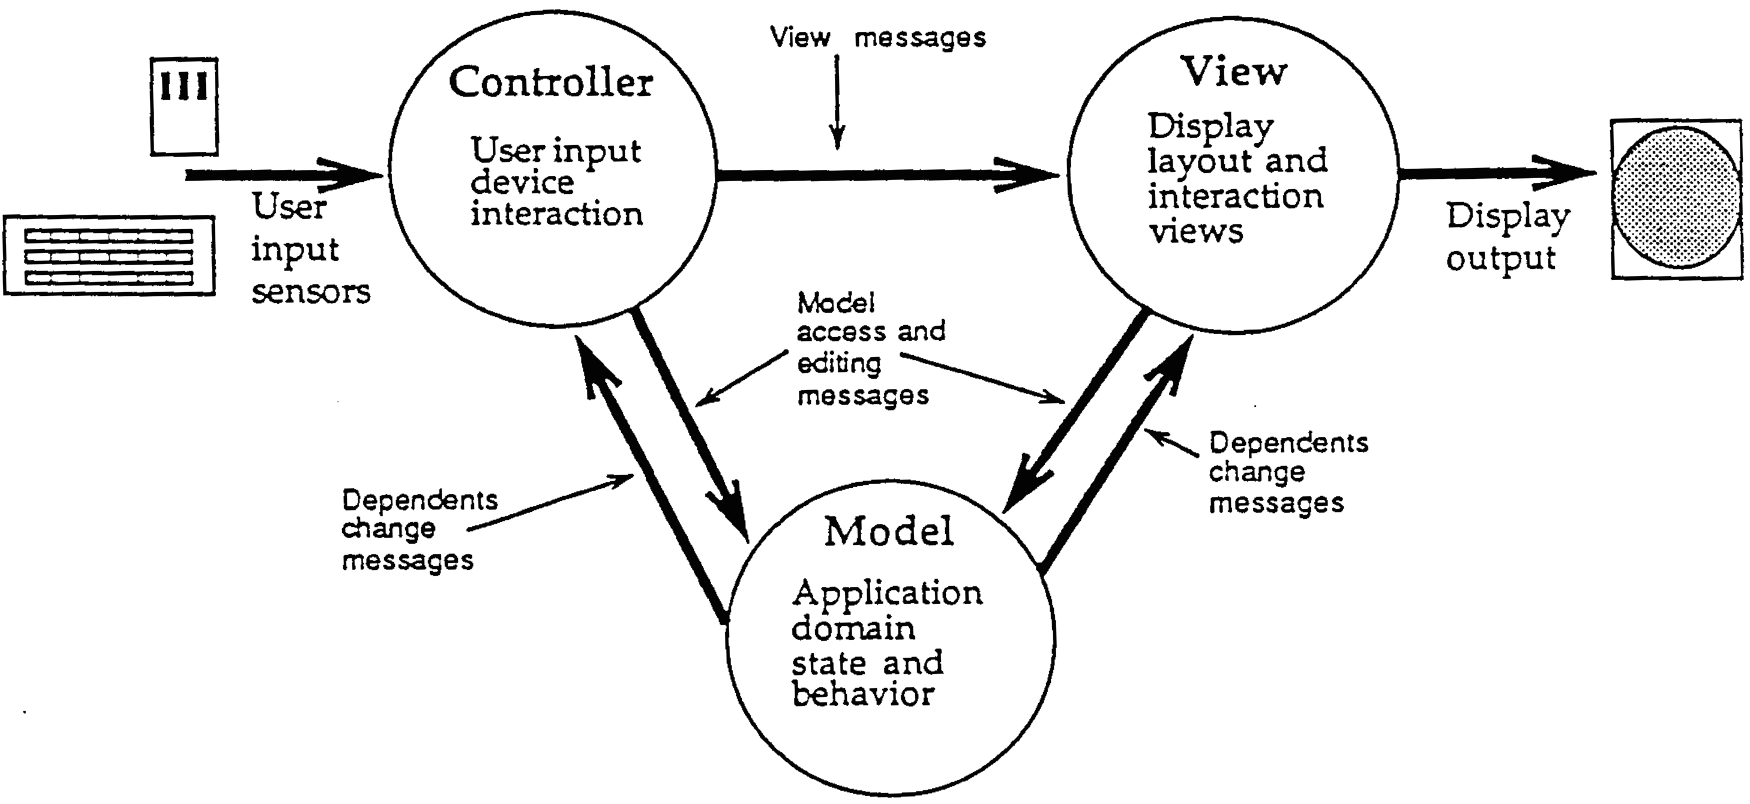
\includegraphics[width=1.0\textwidth]{figures/mvc.png}
\caption[MVC-architecture]{MVC-architecture (Krasner and Pope, 1988)}
\label{fig:mvc}
\end{figure*}
\todo{ TODO krasner and pope 1988: http://heaveneverywhere.com/stp/PostScript/mvc.pdf }

\subsection{Model-View-ViewModel}\label{ref:mvvm}

This architectural pattern, also known as ``Model-View-Binder'', is similar to MVC but puts more emphasis on the seperation between back-end and front-end. It's parts are as follows (and can be seen in fig. \ref{fig:mvvm}):\todo{TODO sources}

\begin{description}
  \item[The model] is the back-end business-logic and state. It can be on a different machine entirely, e.g. a web-server.
  \item[The view-model] contains the front-end logic and state. It is a thin binding layer, that processes inputs and that manages and provides the data required by the view.
  \item[The view] is a stateless rendering of the data retrieved from the view-model; in the case of some frameworks, this happens via declarative statements in the view's templates, that automatically get updated when the data in the view-model changes. User-input events raised in the view get forwarded to the view-model.
\end{description}

\begin{figure*}
\centering
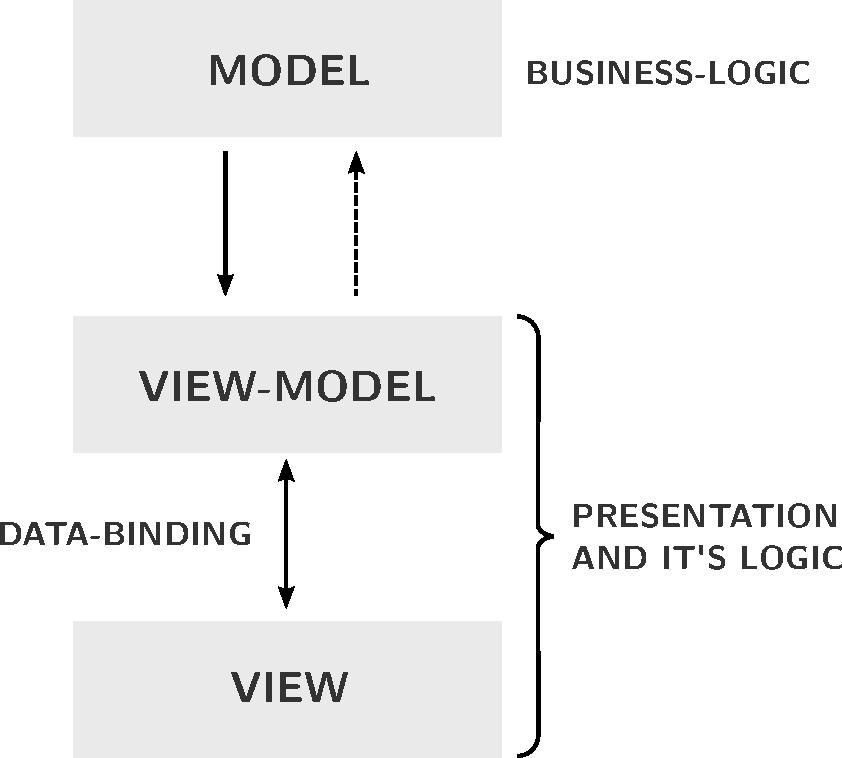
\includegraphics[height=8cm]{figures/mvvm.pdf}
\caption[MVC-architecture]{ MVVM-architecture (diagram \href{https://en.wikipedia.org/wiki/File:MVVMPattern.png}{adapted from wikimedia}\footnotemark{})}
\label{fig:mvvm}}
\end{figure*}
\footnotetext{\url{https://en.wikipedia.org/wiki/File:MVVMPattern.png}}

\subsection{Angular 1.x MVC}\label{ref:angular-mvc}

\todo{Too much detail! Move a lot of these details to later chapters (e.g. "solution » ng best practices" or "solution » why we moved from ng to ng-redux")}

Angular 1.x is a javascript-framework that roughly follows the MVC/MVVM architectures, but has a few conceptual variations and extensions.

On the View-side of things there's templates (see fig. \ref{fig:ng-template} for an example from the webofneeds-codebase). These are either specified in an html-file and then later linked with a controller or are a string in the declaration of something called a "directive" (which are custom html tags or properties). Every template has a scope object bound to it and can contain expressions---e.g. those in curly braces---that have access to that scope object. For the example in fig. \ref{fig:ng-template} this means, that---in the HTML that the user gets to see---the curly braces will have been replaced by the result of \texttt{self.post.getIn(['won:hasContent','won:hasTextDescription'])} (the \texttt{getIn} is there because \texttt{post} is an \fnurl{https://facebook.github.io/immutable-js/}{immutable-js} object). Practically every time the result of that expression changes, angular will update the displayed value. Basically every expression causes a ``watch'' to be created (this can also be done manually via \texttt{\$scope.watch}). On every ``digest-cycle'' checks all of these watch-expressions for changes and then executes their callbacks, which in the case of the curly-braces causes the DOM-update.

Beyond the curly braces, angular also provides a handful of other template-utilities in the form of directives. For instance the property-directive \texttt{ng-repeat} allows iterating over a collection as follows:

\begin{verbatim}
<div ng-repeat="el in collection">{{el.someVar}}</div>
\end{verbatim} 

Or, similiarly, \texttt{ng-show="someBoolVar"} conditionally displays content.

Note that these template-bindings are bi-directional, i.e. the code in the template can change the the values in the scope. Additionally, templates/directives can be nested within each other. By default, their scopes then use javascript's \fnurl{https://developer.mozilla.org/en/docs/Web/JavaScript/Inheritance_and_the_prototype_chain}{prototypical inheritance} mechanism, i.e. if a value can't be found on the template's/directive's scope, angular will then go on to try to get it from the on the one wrapping it (and so on)
This allows writing small apps or components where all data-flows are represented and all code contained in the template. For medium-sized or large apps however, the combination of bi-directional binding and scope inheritance, can lead to hard-to-follow causality, thus hard-to-track-down bugs and thus poor maintainability. More on that later. % in section X
\todo{TODO add reference to that subsection} 
Also, using scope inheritance reduces reusability, as the respective components won't work in other contexts any more. \todo{move critique of bi-dir binding and inheritance to later chapter}

\todo{ TODO get syntax-highlighting to work in figures (see comment in .tex) } % \begin{lstlisting}[style=json]}
\begin{figure*}
\centering
\begin{verbatim}
...
<h2 class="post-info__heading"
  ng-show="self.post.getIn(['won:hasContent','won:hasTextDescription'])">
    Description
</h2>
<p class="post-info__details"
  ng-show="self.post.getIn(['won:hasContent','won:hasTextDescription'])">
    {{ self.post.getIn(['won:hasContent','won:hasTextDescription']) }}
</p>
...
\end{verbatim}
\caption{Excerpt of angular-template}
\label{fig:ng-template}
\end{figure*}

For all but the very smallest views/components the UI-update logic will be contained in angular's controllers, however. They are connected with their corresponding templates via the routing-configuration (more on that later \todo{ref to routing-subsection}) or by being part of the same directive \todo{ref to directive-subsection}. Controllers have access to their template's scope and vis versa %(see section X
\todo{ref to controllerAs discussion}
%)
Theoretically it's possible to pair up / reuse controllers with different templates, but this can lead to hard-to-track-down and I'd advise against doing that.
When nesting templates and thus they're associated controllers, actually it's the controllers that form the prototypical inheritance chain. Thus, if a variable isn't found on the controller respectively it's scope, the default is to check on it's parent('s), up to the root-scope. Note that scopes can be defined as isolated in the routing config \todo{ref to routing/isolated-scope section} to avoid this behaviour, which I'd recommend for predicatability- and thus maintainability-reasons.

\todo{ can be reused with different template, but that rarely happens and tends to lead to hard-to-track-down bugs.}
\todo{nesting templates (not directives?)---how does it work anyway?}

\todo{move controllerAs advice to later chapter}
\begin{comment}
Controllers have access to their template's scope via the variable \texttt{scope} that they get in their factory-function/constructor. 
Alternatively, they can be bound e.g. as \texttt{self} to the scope by specifying \texttt{controllerAs: "self"} in the routing-/directive-config. This avoids the situation where you specify a variable on the wrong object and then the template-expression can't find it (e.g. if you miss that \texttt{this} in a bound function points to the controller-object instead of the scope) Generally speaking, using \texttt{controllerAs} makes mistakes/bugs less likely. 
\end{comment}

Now, with models/scopes, views/templates and controllers we would have a classical MVC-framework (see section \ref{ref:mvc}). However, angular also has the concept of services: Essentially, they are objects that controllers can access and that can provide utility functions, manage global application state or make http-requests to a web-server. Controllers can't gain access to each other---except for nesting / prototypical inheritance---but they can always request access to any service (via dependency injection; more on
that later\todo{ref to subsection}). Examples of services are \texttt{\$scope} that, amongst others, allows registering custom watch-expressions with angular outside of templates (see fig. \ref{fig:ng-simple-ctrl} for an example). Another example for a service would be our custom \texttt{linkeddata-service.js} that can be used to load and cache RDF-data\footnote{see section \ref{data-on-won-nodes} for more on RDF}.


\todo{ TODO get syntax-highlighting to work in figures (see comment in .tex) } % \begin{lstlisting}[style=javascript]}
\begin{figure*}
\centering
\begin{verbatim}
var myApp = angular.module('myApp', []);
myApp.controller('PostController', function ($scope) {
  $scope.post = { text: 'heio! :)' };
  $scope.$watch('post.text', function(currentText, prevText) {
    console.log('Text has been edited: ', currentText);
  });
});
\end{verbatim}
\caption{Example of a very simple controller and usage of the \texttt{\$scope}-service}
\label{fig:ng-simple-ctrl}
\end{figure*}

With services added to the mix, we can also view the angular framework through the lense of MVVM (see section \ref{ref:mvvm}), with templates as views, scopes and controllers as view-models and services as models or as proxies for models on a web-server (as we did with the \texttt{linkeddata-service.js}).

% \todo{ TODO get syntax-highlighting to work in figures (see comment in .tex) } % \begin{lstlisting}[style=javascript]}
\begin{figure*}
\centering
\begin{verbatim}
myApp.config(['$routeProvider',
  function($routeProvider) {
    $routeProvider.
      when('/landingpage?:focusSignup', {
        templateUrl: 'app/components/\
          landingpage/landingpage.html',
        controller: 'LandingpageController'
      }).
      when('/post/?postUri', {
        templateUrl: 'app/components/\
          post/post.html',
        controller: 'PostController'
      }).
      otherwise({
        redirectTo: '/landingpage'
      });
  }]);
\end{verbatim}
\caption{Example of routing-configuration in Angular 1.X}
\label{fig:ng-simple-routing}
\end{figure*}

% todo move this to later chapters (e.g. a section on module systems)

Note, that Angular 1.x uses it's own module system to manage directives, controllers and services. If you include all modules directly via \texttt{<script>}-tags in your \texttt{index.html}, this mechanism makes sure they're executed in the correct order. However, this also means, that if you want to combine all your scripts into one \texttt{bundle.js}\footnote{
Bundling for instance helps to reduce the number of HTTP-requests on page-load and thus it's performance. It can be done by using a build-tool like browserify, webpack or jspm plus a module system like AMD, CommonJS or the recently standardized ES6-modules (see \url{http://www.ecma-international.org/ecma-262/6.0/#sec-imports})}
}
you'll have to specify the same dependencies twice---once for your bundling module system and once for angular's, as can be seen in figure \ref{fig:ng-duplicate-dependencies}.\todo{ref number doesn't match figure's}

\begin{figure*}
\centering
\begin{verbatim}
/* es6 imports for bundling */

import angular from 'angular'
import createNeedTitleBarModule from '../create-need-title-bar';
import posttypeSelectModule from '../posttype-select';

//...

class CreateNeedController { /* ... */ }

//...

/* angular module declaration */

export default angular.module(
  /* module's name: */
  'won.owner.components.createNeed', 
  [ /* module's dependencies: */
    createNeedTitleBarModule,
    posttypeSelectModule,
    // ...
  ])
  .controller(
    'CreateNeedController', 
    [
      '$q', '$ngRedux', '$scope', // services for ctrl
      CreateNeedController // controller factory/class
    ])
.name;
\end{verbatim}
\caption{Example of module- and controller-declaration in \texttt{create-need.js}}
\label{fig:ng-duplicate-dependencies}
\end{figure*}

\todo{TODO reference ng docu}

\begin{comment}

    * [ ] views - templates + controller
	* [ ] controllers / factory methods
        * [x] somewhere between MVVM-viewmodels and MVC-controllers
		* [ ] best practice: avoid putting too much code into these
	* [ ] routing 
        * [ ] how controllers+html-templates are brought together
    * [ ] directives (component style or attributes)
        * [ ] explain with example of modal?
        * [ ] preferable to view+controller as code for both + bundling of them is in one place (~react components)
    * [x] services ~MVVM-model
    * [x] arguably more mvvm than mvc
    * [ ] rather steep learning curve. 
        * [ ] especially to use it well. there's many pitfalls for people just starting out with it to produce a code-base that's hard to maintain later on. (personal experience with smartengine-code and own code)
        * [ ] TEXT?: as concrete usage example angular solves a wide range of different problems (routing, state managment, networking, display,...) and it does so with an equally wide range of mechanisms. Redux on the other hand, has one a very small number of mechanisms, that it uses to solve all these problems similiarly (e.g. routing-information is part of the redux-state)
        * [ ] TEXT: ... As you can see angular is rather complex in it's architecture and contains quite a few pitfalls for the unwary newcomer. As such, it has a rather steep learning curve.
    * [x] bi-directional binding
    * [ ] auto-injection into scope via things like ng-model
    * [x] scoping / hierarchy of controllers
    * [x] scope-inheritance and it's problems!
    * [ ] modules and dependency-injection
      * [ ] "Bringing it all together..."
      * [ ] need to include each and every javascript file (in the right order?). everything is loaded with quite a few http-requests. can be bundled though
        * make sure to use strict mode to allow bundling
      * [ ] no tree-shaking
      * [x] redundant to es6-module system
    * [x] services
      * [x] keep global state
      * [x] wrap access utilities to server-APIs
      * [x] access to utility functions that can be injected (instead of being attached to the window)
    * [ ] controllers
      * [x] both controllers and partly models (is angular actually mvvm?)
      * [x] can be reused with different template, but that rarely happens and tends to lead to hard-to-track-down bugs.
      * [ ] mostly used at view level. below that directives provide more atomic bundling of template and code.
    * [x] templates
    * [ ] filters
      * { probably not necessary to explain }
    * [ ] directives
      * [ ] bundle controller and template in one file
      * [ ] register custom html-tag (unless used in attribute, like ng-show/-class/-..., or class mode)
    * [ ] routing
      * [ ] html-fragments
      * [ ] ui-router (?) (are we using or have we used it?)
\end{comment}

\subsection{Meteor}

\todo{ dunno if necessary? }

\subsection{React}

React is a framework that specifically provides the view (and potentially view-model) of application architectures. It provides a mechanism to define custom components/HTML-tags (comparable to directives in Angular 1.X and webcomponents in general) as a means to achieve seperation of concerns and code reusability. These components are stateful and contain their own template code, usually specified in the form of inline-HTML (that's processed to calls to the React-libary---more on that
below). % see $x / at the bottom of this section for an example of $y, were it written as React-component % TODO take short directive from won-codebase and translate it to React
For all but the smallest applications---where the state can be fully contained in the components---you'll need some extra architecture additional to React, for instance to handle the application-state or manage HTTP-requests and websockets. This is usually where Flux (see section \ref{ref:flux}) and Redux (see section \ref{ref:redux}) come in.

In any way, to get to the bottom of what distinguishes React, one should first start by talking about the big problem of the Document Object Model: When there's a large number of nodes on the screen, manipulating several quickly one after each other can take quite a while, causing the whole interface to noticeably lag as every changed node causes a reflow of the layout and rerendering of the interface. React is the first of a row of libraries to use a light-weight copy of the DOM (called ``Virtual DOM''). The idea is to only directly manipulate the VDOM and then apply
the differential / cumulative change-set to the actual DOM in one go. This means a performance gain where multiple operations are applied to the same node or multiple nodes at the same time as React makes sure that the slow reflow and rerendering only happens once. From a development side of things, this diff'ing-process means, that there's no need to manage DOM-state-changes and intermediate states; the template-code in the components can be written, as if they were rendered completely new every cycle, i.e. only a direct
mapping from data to desired HTML needs to be provided and React handles the changes to get there.

As a notable difference to Angular, React's data-flow is unidirectional, meaning a component can read the data it gets via it's html-tag-properties, but it can't modify them. This is a useful guarantee, to avoid bugs like when you use a component, don't know it modifies it's parameter variables (intentionally or as a bug) and thus influences your unsuspecting parent component as a side-effect. Intended child-to-parent communication can be done explicitly via events published by the child (or via callback functions). 

\begin{comment}
class Square extends React.Component {
  constructor() {
    super();
    this.state = {
      value: null,
    };
  }
  render() {
    return (
      <div className="square">
		{this.props.myproperty}
		{this.state.value}
      </div>
    );
  }
}
\end{comment}

\subsection{Flux}\label{ref:flux}

When you start reading about React you'll probably stumple across Flux rather earlier than later. It is the architecture popularized alongside of React and akin to MVC in that it seperates handling input, updating the state and displaying the latter.

However, instead of having bi-directional data-flow between the architectural components, Flux' is uni-directional and puts most of it's business logic into the stores that manage the state. To give an example of a flow through this loop: Say, a user clicks on a map widget with the intend of picking a location. The widget's on-click method, would then create an object that's called an action that usually contains type-field like \texttt{"PICK\_LOCATION"} and any other data describing the
user-interaction like geo-coordinates. It then goes on to pass the action object to the globally available dispatcher, that broadcasts it to all stores. Every store then decides for itself in what way it wants to update the data it holds. For instance, a \texttt{locationStore} could updated the geo-coordinates it holds. The stores would then go on to notify all components that are listening to them in particular that their state has changed (but not in what way). The affected
components, e.g. the map and a text-label below it, poll the store for the data and render themselves anew (as if it was the first time they were doing this)---e.g. the map would place a singular marker on the coordinates it gets from the store and the label would write out the coordinates as numbers.

Because of the last point---the components rendering themselves "from scratch" every time, i.e. them being an (ideally) state-less mapping from app-state to HTML---this architecture pairs well with React's VDOM.

When there's preprocessing that needs to be done on the data required for the action-object---e.g. we want to resolve the geo-coordinates to a human-friendly address-string---action-creators are the usual method to do so. These are functions that do preprocessing---including HTTP-requests for instance---and then produce the action-objects and dispach them. 

Though being an architecture, i.e. a software-pattern,  per se, usually one will use one of many ready made dispatchers and also a store-prototype to inherit from, that will reduce the amount of boilerplate code necessary to bootstrap a Flux-based application.

Stores can have dependencies amongst each other. These are specified with a function along the lines of \texttt{B.waitFor(A)}, meaning that the store B only starts processing the action once A has finished doing so. Managing these dependencies in a medium-sized to large application can be quite complex, which is where Redux (see below) tries to improve over Flux.

In general, using Flux profits from using immutable data-structures for the state (e.g. those of \fnurl{https://facebook.github.io/immutable-js/}{immutable-js}). Without these, components could accidentally modify the app-state by changing fields on objects they get from the stores, thus having the potential for hard-to-track-down bugs.
 
\begin{comment}
% TODO image !!!!

  * [ ] quite a learning-curve
  * [x] actions
  * [x] dispatcher
    * [x] there are many different implementations of these (the one by fb, the one by yahoo,...)
  * [x] stores
    * [x] waitFor
    * [x] dependencies between these can be hard to understand
    * [ ] lot of overhead
  * [x] views
    * [ ] most dispatchers / setups are geared to be used with redux
\end{comment}


\subsection{Redux}\label{ref:redux}

The developers/designers of Redux list the object-oriented Flux- (see above) and functional Elm-architecture (see below) as \fnurl{http://redux.js.org/docs/introduction/PriorArt.html}{prior art}. It mainly differs from Flux, by eschewing the set of stateful stores, for the Elm-like solution of having a single object as app-state, that a single reducer-function \texttt{(state, action) => state'} gets applied to for every new action, thus updating the state. As such there's also formally no need for a
dispatcher, as there's only a single function that's updating the state. Seperation of concerns---that Flux achieves with it's larger number of stores---can be achieved in Redux by having the reducer function call other functions, e.g. one per subobject/-tree of the state. 

As the simplest implementation of this architecture consists of only a single function and a component that feeds actions into it, the learning curve is relatively shallow compared to Flux and almost flat compared to Angular's MVC.

Redux profits from immutable data-structures for the app-state almost even more than Flux. The reducer function is supposed to be stateless and side-effect free (i.e. pure). In this particular case this means that parts of the system, that still hold references to the previous state, shouldn't be influenced by the state-update. If they want the new state, they'll get notified through their subscription. Using immutable data guarantees this side-effect freeness to some extend (nothing can
prevent you from accessing the global \texttt{window}-scope in javascript though, so ideally don't do that). This property also means, that you should try to move as much busieness logic as possible to the reducer, as it's comparatively easy to reason about and thus debug. For all things that require side-effects (e.g. anything asynchronous like networking) action-creators are the go-to solution---same as in Flux.


\begin{comment}
    % TODO graphic
  * [x] http://redux.js.org/
  * [x] can be super-simple (give trivial example)
  * [x] easy to learn (it's only one event-bus/dispatcher, one reduction-function)
  * [x] ideally used with immutable data for model (to avoid bugs due to pass-by-reference and later modification)
  * [x] doesn't deal with side-effects by default (see ACs and actors later)
  * [x] (action-creators (for pre-processing))
  * [x] actions
  * [x] dispatcher
  * [x] seperation of concerns by having subfunctions for reducer
  * [x] reduction function
    * [x]  synchronous (can't do asynch side-effects here)
    * [x] (supposed to be) side-effect free. do as much as business logic as possible here.
 * [x] components
\end{comment}

\subsection{Ng-Redux}\label{ref:ng-redux}

\fnurl{https://github.com/angular-redux/ng-redux}{Ng-Redux} is framework that's based on the Redux-architecture and is geared to be used with Angular applications. The latter then handles the Components/Directives and their updates of the DOM, whereas Ng-Redux manages the application state. In this combination, the frameworks binds functions to the angular controllers to trigger any of the available actions. Even more importantly, it allows registering a \texttt{selectFromState}-function that gets run after
the app-state has been updated and which' result is then bound to the controller. It also provides a plugin/middleware-system for plugins that provide convienient use of asynchronicity in action-creators (through ``thunk'') or keeping the routing information as part of the application state (through the ``ngUiRouterMiddleware'').

\begin{comment}
    % TODO example of use in a simple directive?
  * [ ] good for migrating (why we chose it)
  * [x] duplicate imports if using es6 (though not ng-redux inherent)
  * [ ] explain binding into routing, setup of watches, importance of one way bindings
  * [ ] has a dispatcher (what does it do? it should be super minimal)
\end{comment}


\subsection{Elm-Architecture}

\fnurl{http://elm-lang.org/}{Elm} is a functional language who's designers set out to create something as accessible to newcomers as Python or Javascript. It can be used to build front-end web application (browser-less execution in node is currently being worked on). The original Elm-architecture was based on functional reactive programming---i.e. using streams/observables like CycleJS' MVI (see below) that it inspired as well---but they have since been removed to make it more accessible to
newcomers. The \fnurl{https://guide.elm-lang.org/architecture/}{current
architecture}, in it's basic form, requires one to define the following three functions and pass them to Elm's \texttt{Html.beginnerProgram} (that runs the app):


\begin{enumerate}
    \item \texttt{model : Model}, that initializes the app-state.
    \item \texttt{update : Msg -> Model -> Model}, which performs the same role as \texttt{reduce} in Redux, with \texttt{Msg}s in Elm being the equivalent to actions in Redux.
    \item And lastly, \texttt{view : Model -> Html Msg} to produce the HTML from the model.
\end{enumerate}

As Elm is a pure/side-effect free language, these can't handle asynchronity yet (e.g. HTTP-requests, websockets) or even produce random numbers. The full architecture, that handles these, looks as follows (and is run via \texttt{Html.program}):

\begin{enumerate}
    \item \texttt{init : (Model, Cmd Msg)} fulfills the same role as \texttt{model}, but also defines the first \texttt{Cmd}. These allow \textit{requesting} for side-effectful computations like asynchronous operations (e.g. HTTP-requests) or random number generation. The result of the \texttt{Cmd} is fed back as \texttt{Msg} to the next \texttt{update}.
    \item the function \texttt{update : Msg -> Model -> (Model, Cmd Msg)} now also returns a \texttt{Cmd} to allow triggering these depending on user input or the results of previous \texttt{Cmd}s. This allows keeping all of the business-logic in the \texttt{update}-function (as compared to Flux'/Redux' action-creators) but trades off the quality, that every user-input or websocket message can only trigger exactly one action and thus exactly one update (thus making endless-loops
        possible again)---arguably this is a rather neglible price.
    \item \texttt{subscriptions : Model -> Sub Msg} allows to set up additional sources for \texttt{Msg}s beside user-input, things that \textit{push}---if you so will---
e.g. listening on a websocket.
    \item \texttt{view : Model -> Html Msg} works the same as in the simple variant.
\end{enumerate}

\begin{comment}
    % TODO snippet / pic of previous 
    * [x] previous (at time of designing)
    * [x] current
\end{comment}

\subsection{CycleJS MVI}

CycleJS is an 'functional reactive programming'-based framework, which Model-View-Intent architecture is structured similar to the Redux- and (original) Elm-architectures. 

But first: The framework itself is based on functional reactive programming (FRP) and uses observables/streams of messages for it's internal data-flows. Think of them as Promises that can trigger multiple times, or even more abstract, pipes that manipulate data that flows through them and that can be composed to form a larger system. The integral part developer's using the framework need to specify is a function \texttt{main(sources) => ({ DOM: htmlStream})} (see fig. \ref{fig:cyclejs}) that takes a driver ``\texttt{sources}'') like the DOM-driver that allows creating stream-sources (e.g. click events on a button). One would then apply any data-manipulations in the function and return a stream of virtual DOM. In the very simple example of fig. \ref{fig:cyclejs} for every input-event a piece of data/message would travel down the chained functions and end up as a virtual DOM object. This \texttt{main}-function is passed to \texttt{run} to start the app.

% TODO syntax highlighting
\begin{figure*}
\centering
\begin{verbatim}
import {run} from '@cycle/xstream-run';
import {div, label, input, hr, h1, makeDOMDriver} from '@cycle/dom';

function main(sources) {
  const sinks = {
    DOM: sources.DOM.select('.field').events('input')
      .map(ev => ev.target.value) // get text from field
      .startWith('') // initial value / first stream-message
      .map(name =>
        div([
          label('Name:'),
          input('.field', {attrs: {type: 'text'}}),
          hr(),
          h1('Hello ' + name),
        ])
      )
  };
  return sinks;
}

run(main, { DOM: makeDOMDriver('#app-container') });
\end{verbatim}
\caption{CycleJS hello-world example from \url{https://cycle.js.org/}}
\label{fig:cyclejs}
\end{figure*}

For more complex applications, an architecture similiar to Redux/Elm, called ``Model-View-Intent'', is recommended. For this, the stream in \texttt{main} is split into three consecutive sections: 

\begin{enumerate}
\item Intent-functions that set up the input streams from event-sources (e.g. DOM and websockets) and return ``intents'', that are equivalent to Flux'/Redux' actions and Elm's messages.
\item The model-stage is usually implemented as a function that is \texttt{reduce}'d over the model (equivalent to how Redux deals with state-updates)
\item And lastly the view-stage takes the entire model and produces VDOM-messages.
\end{enumerate}

Seperation of concerns happens by using sub-functions or splitting the stream at each stage (or starting with several sources in the first) and combining them at the end of it.

\begin{comment}
* [ ] driver's are similiar to actors?
\end{comment}

\chapter{Methods}

\begin{comment}
  <blockquote>
Methodik, die verfolgt wurde, um Lösung zu entwickeln
 -> ich glaube, den Hevner Artikel (Design Science in Inf Sys research) habe ich dir eh geschickt, eignet sich als Methode. Verbinde einfach sein abstraktes Konzept mit dem, was du tatsächliche gemacht hast (was war die Ausgangssituation (Legacy code mit Angular), wie hat dein Suchprozess ausgesehen (wie bist du auf react gekommen, was waren die Alternativen,...), Was kam aus der globalen Knowledge Base (react), wie kamst du zu deiner Synthese aus react+rdfstore-js+angular)
 </blockquote>

 <blockquote>
 in the method chapter you should explain:
* hevner
* RDF, linked data, JSON-LD
* angular
* flux/redux
 </blockquote>

 % Flo @ hevner-summary: good first note sheet. You can convert that into a 1-2 page intro of the methods section. Then you go on to show how you applied this framework, effectively proving that what you did is research, and not engineering.

 % TODO better describe/address the figure

% 2: @hevner-länge: macht nichts, aber man darf sich beim lesen nicht fragen, warum du einem das erzählstFrom:phlow_06 (Flo SAT)wenn du keinen grund dafür findest: weglassen. sonst: sagen. -- dh ich sollte e.g. auch nur die artefakt-kategorie beschreiben, unter die der prototyp / die architektur fällt, bzw die methoden, die tatsächlich verwendet wurden?(die guidelines werde ich alle brauchen, da die dann hinterher ja die struktur für den kern-teil darstellen sollen). wobei die anderen artefakt-kategorien/-abgrenzung ermöglichen --> liste an methoden kürzen

% dann bleibt das eigentlich eh bei den 3-4 seiten (atm ist es eh fast nur aufzählung + kurze definition für alles)
% From:phlow_06 (Flo SAT) genau, es fehlt glaub ich noch die erklärung, warum das jetzt aufgezählt wird - also wie du das für dich umsetzt

% TODO answer the two fundamental questions explicitly

<!--

Vorlage: Arbeit vom Roman?

## Ressources

### Redux

<https://medium.com/javascript-scene/10-tips-for-better-redux-architecture-69250425af44#.auuzhdjz3>
[You Might Not Need Redux](https://medium.com/@dan_abramov/you-might-not-need-redux-be46360cf367#.2xg3p7aef)


<!-- TODO see hevner_summary + notes !!!! -->
<!--
TODO
Technische Realisierung / solutions
  * follow hevner's structure(?)
-->
<!--
describe architecture / redux cycle here
describe entire tool-chain?
-->


From TU-outline:
* used concepts
  * redux
  * side-effects / immutable data
  * bi-directional binding
* methods and/or models
* languages
  * javascript
  * sparql?
  * json-ld
* design methods
  * hevner
  * iterations / design-cycle
* data models
* analysis methods
  * ???
  * personal experience / experience of colleagues?
* formalisms

\end{comment}

\section{Design Science in Information Systems Research}

For the work preceding this thesis the methodological
framework presented in ``Design Science in Information
Systems Research'' by Hevner et al (2004) was used.
I'll try to give a short overview over it in this section.

\subsection{Design Science}

The paper states that a lot of the research surrounding information systems can be described as design- and/or behavioral science.

It roughly defines \textbf{behavioral science} with regard to IS-research as concerned with the analysis of the interactions of people and technology, with the goal of uncovering ``truths'' and predicting or explaining phenomena surrounding these interactions.

In comparison, Hevner et al describe \textbf{design science} as concerned with problem solving and construction with the background that doing so leads to understanding the addressed ``wicked'' problem \footnote{\label{ref:wicked}Here, ``wicked'' problems (Brooks 1987, 1996; Rittel, Webber 1984) are defined as those with unstable requirements, ill-defined environmental contexts, complex interactions among subcomponents of problem and solution, an inherent flexibility to change design processes and artifacts and a critical dependence on human cognitive abilities (e.g. creativity) and social abilities (e.g. teamwork) for effective solutions}. It diffentiates itself from \textbf{routine design} by addressing problems without existing best-practices/requisite knowledge and solves them unique/innovative ways, or improves efficiency. By doing so, new knowledge is contributed to the foundations and methodolgies. Design-science usually also produces prototypes instead of full-grown systems.



% TODO replace references to wicked problems with glossary entry
% foobar \glspl{wicked}
% \newglossaryentry{wicked}
% {
  % name={wicked problem},
  % description={These are defined in  Brooks 1987, 1996 and Rittel, Webber 1984 as problems with unstable requirements, ill-defined environmental contexts, complex interactions among subcomponents of problem and solution, an inherent flexibility to change design processes and artifacts and a critical dependence on human cognitive abilities (e.g. creativity) and social abilities (e.g. teamwork) for effective solutions}
% }

The paper also presents two \textbf{fundamental questions} of design research as ``What utility does the new artifact provide?'' and ``What demonstrates that utility?''. As all other's from Hevner et al (2004) that are referenced or quoted here, they'll be addressed in the next chapter. %TODO more concrete/pinpointed reference

\subsection{Design Processes and Artifacts}


March and Smith (1995)\footnote{TODO} list two processes involved in design, \textbf{build/generate} and \textbf{evaluate}, that form a cycle (see figure \ref{fig:hevner}). They differentiate the artifacts produced as:

\begin{description}
 \item[constructs] that provide the language to define problems and solutions (e.g. programming languages)
 \item[models] that abstract and represent these and allow exploring the effects of design decisions
 \item[methods] that define how to solve problems or aid with searching the problem-space (e.g. algorithms, best practices)
 \item[instantiations] that demonstrate feasibility and enable assessing suitability for the intended purpose
\end{description}

\subsection{Design-Science Research Guidelines}

\begin{figure*}
\centering
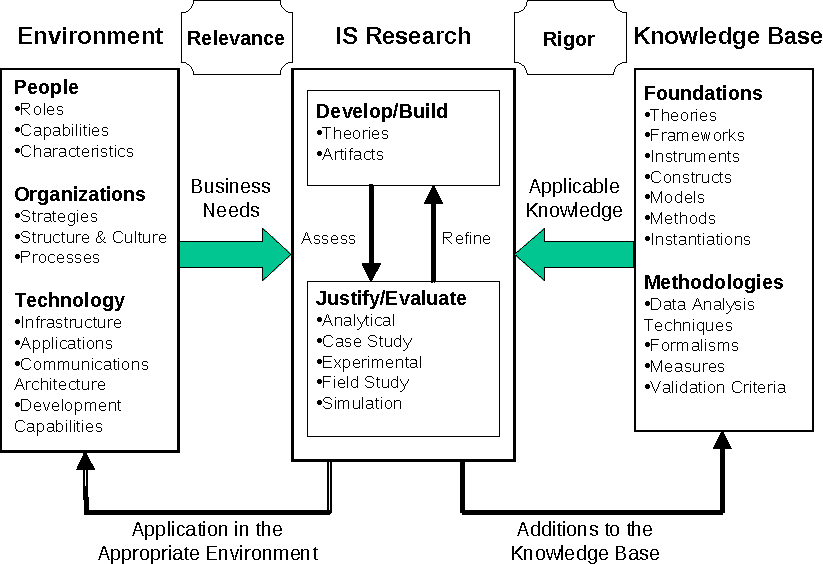
\includegraphics[width=1.0\textwidth]{figures/Hevner-et-al-2004-figure-2.pdf}
\caption{\label{fig:hevner}Information Systems Research Framework (Hevner et al 2004)}
\end{figure*}

Hevner et al (2004) defines seven guidelines that design-science in information systems should address (but not necessarily come-what-may adhere to), which will be done in the next chapter. % TODO more conrete/clickable reference
They are as follows:

% TODO
% \begin{leftbar}
%  asdf
%  asdf
%\begin{leftbar}

%\begin{siderules}
%\begin{quotation}
\begin{description}

\item[Design as an Artifact]
``Design-science research must produce a viable artifact in the form of a construct, a model, a method, or an instantiation.'' This allows to demonstrate feasibility -- for cases where that wasn't a given yet -- thus making it research (as opposed to routine design).

% This

\item[Problem Relevance]
``The objective of design-science research is to develop technology-based solutions to important and relevant business problems.'' Relevancy here is with respect to a  ``constituent community'' (e.g. IS practitioners)
% TODO mention Technology Acceptance Model here (and need to define it)? i haven't really done anything based on it, so whatever

\item[Design Evaluation]
``The utility, quality, and efficacy of a design artifact must be rigorously demonstrated via well-executed evaluation methods.'' This usually requires integration into the usage context (to see if it ``works'' there or is ``good'' in it), the definition of appropriate metrics and gathering of appropriate data. Evaluation provides valueable and necessary feedback for the design iterations (see figure \ref{fig:hevner})

\item[Research Contributions]
``Effective design-science research must provide clear and verifiable contributions in the areas of the design artifact, design foundations, and/or design methodologies.'' Important here is the novelty of the artifact -- by extending or innovatively (re-)applying previous knowledge -- as well as its generality and significance.

\item[Research Rigor]
``Design-science research relies upon the application of rigorous methods in both the construction and evaluation of the design artifact.'' This means applying existing foundations and methodologies, using effective metrics and formalising. Note, however, that an overemphasis on rigor can often lead to lower relevance (Lee 1999), as many environments and artifacts defy an excessive formalism (see ``wicked problems'' at footnote \ref{ref:wicked}). %TODO better reference / use glossary entry

\item[Design as a Search Process]
``The search for an effective artifact requires utilizing available means to reach desired ends while satisfying laws in the problem environment.'' This entails using heuristic search stragegies (e.g. best-practices as starting point) in ght generate/test-cycle (see figure \ref{fig:hevner}) However, again, it might not be possible to formalize or even determine any of these, due to the ``wicked'' (see footnote \ref{ref:wicked}) nature of tackled problems. As a result it might often be necessary to only work on simpler sub-problems, giving up relevancy in turn.

\item[Communication of Research]
``Design-science research must be presented effectively both to technology-oriented as well as management-oriented audiences.'' For the former the construction and evaluation process are important (e.g. to allow reproduction). For the latter the question boils down to ``Is it worth the effort to use the artifact for my business?''. This can be broken down as ``What knowledge is required?'' respectively ``Who can use it?'', ``How imporant is the problem?'', ``How effective is the solution?'' as well as some details in appendicesto appreciating the work.

\end{description}
%\end{quotation}
%\end{siderules}



\subsection{Design Evaluation Methods}

\begin{comment}
% TODO drop methods that weren't used

% TODO metrics from "Design Evaluation:"
  * evaluate in terms of:
    * functionality
    * completeness
    * consistency
    * accuracy
    * performance
    * reliability
    * usability
    * fit with the organization
    * other relevant quality attributes
* establish if it does work and in which environments
  * what constitutes “working” and “good”? which metrics?
  * compare with other solutions for the same problem by human experts
\end{comment}

Observational methods:

\begin{description}
  \item[Case Study] ``Study artifact in depth in business environment''
    % * **{** ^ that **}**
    % * **{** anecdotal evidence by fsu/fk/sbyim/yp how they feel about it? (super-biased due to interaction with me) **}**
  \item[Field Study] ``Monitor use of artifact in multiple projects''
    % * **{** the meinkauf app! what did we use there? ionic and vanilla angular or ng-redux too? <!-- TODO get copy of mk repo --> **}**
\end{description}

Analytical methods:

\begin{description}
  \item[Static Analysis] ``Examine structure of artifact for static qualities (e.g., complexity)''
    % * **{** graph out dependencies in both apps, if necessary in one vertical slice of one process <!-- TODO make graph of dependencies -->  **}**
    % * **{** code-examples of very simple apps with both architectures to demonstrate boiler-plate / overhead? Todo-MVC? <!-- TODO write examples -->  **}**
  \item[Architecture Analysis] ``Study fit of artifact into technical IS architecture''
    % * **{** analyze how well it interacts with the rest of the WoN-ecosystem. what defines “interacts well”? <!-- TODO ponder --> **}**
  \item[Optimization] ``Demonstrate inherent optimal properties of artifact or provide optimality bounds on artifact behavior''
  \item[Dynamic Analysis] ``Study artifact in use for dynamic qualities (e.g., performance)''
\end{description}

Experimental Methods:

\begin{description}
  \item[Controlled Experiment] ``Study artifact in controlled environment for qualities (e.g., usability)''
  \item[Simulation] ``Execute artifact with artificial data''
\end{description}

Testing:

\begin{description}
  \item[Functional (Black Box) Testing] ``Execute artifact interfaces to discover failures and identify defects''
  \item[Structural (White Box) Testing] ``Perform coverage testing of some metric (e.g., execution paths) in the artifact implementation''
\end{description}

Descriptive Methods:

\begin{description}
  \item[Informed Argument] ``Use information from the knowledge base (e.g., relevant research) to build a convincing argument for the artifact’s utility''
    % * **{** ^ this **}**
    % TODO: ^ (only) usable for more innovative artifacts for which other methods aren’t feasible
  \item[Scenarios] ``Construct detailed scenarios around the artifact to demonstrate its utility''
\end{description}

% \input{03_02.tex}

\chapter{<Core>}

\section{Design as an Artifact}
``Design-science research must produce a viable artifact in the form of a construct, a model, a method, or an instantiation.'' This allows to demonstrate feasibility -- for cases where that wasn't a given yet -- thus making it research (as opposed to routine design).

% This

\section{Problem Relevance}
``The objective of design-science research is to develop technology-based solutions to important and relevant business problems.''

% Relevancy here is with respect to a  ``constituent community'' (e.g. IS practitioners)
% TODO mention Technology Acceptance Model here (and need to define it)? i haven't really done anything based on it, so whatever

\section{Design Evaluation}
``The utility, quality, and efficacy of a design artifact must be rigorously demonstrated via well-executed evaluation methods.''
% This usually requires integration into the usage context (to see if it ``works'' there or is ``good'' in it), the definition of appropriate metrics and gathering of appropriate data. Evaluation provides valueable and necessary feedback for the design iterations (see figure \ref{fig:hevner})

\section{Research Contributions}
``Effective design-science research must provide clear and verifiable contributions in the areas of the design artifact, design foundations, and/or design methodologies.''
% Important here is the novelty of the artifact -- by extending or innovatively (re-)applying previous knowledge -- as well as its generality and significance.

\section{Research Rigor}
``Design-science research relies upon the application of rigorous methods in both the construction and evaluation of the design artifact.''
% This means applying existing foundations and methodologies, using effective metrics and formalising. Note, however, that an overemphasis on rigor can often lead to lower relevance (Lee 1999), as many environments and artifacts defy an excessive formalism (see ``wicked problems'' at footnote \ref{ref:wicked}). %TODO better reference / use glossary entry

\section{Research Rigor}
``Design-science research relies upon the application of rigorous methods in both the construction and evaluation of the design artifact.''
% This means applying existing foundations and methodologies, using effective metrics and formalising. Note, however, that an overemphasis on rigor can often lead to lower relevance (Lee 1999), as many environments and artifacts defy an excessive formalism (see ``wicked problems'' at footnote \ref{ref:wicked}). %TODO better reference / use glossary entry

\begin{comment}

## Process

<!--
Flo: "I think it's interesting to describe the actual process, but you should not over-emphasize it. In the end, you came up with a design and an implementation, and that is the artifact you produced.

If you can show multiple iterations of your artifact with 'experiments' evaluating its appropriateness and refinements, fine - but don't zoom into the microscopic level (first I read this, then that, ...).

"

**argument:** feasibility wasn't clear to begin with!!! -> it's research

-->

1. peacemems notifies me of react
2. reading that, i also stumbled across flux
  * flux-article talks about problems with angular/bi-directional data-bindings resonates (same problems when debugging prev prototype) (?)
4. new ulf screens → we’ll need to rewrite (?)
4. rewriting with the old angular setup (angular 2 isn’t production ready)
4. pre-compilation (js, scss) and bundling setup
  * we also switched away from bootstrap, as we'd need to modify it’s styles that heavily anyway
4. actually: when stores and synching via the ws became a thing, started researching flux, ended up stumbling across redux (#342)
  * apparently, we were using flux even before that (see #342). it’s part of a commit from 23 Sep 2015 (1395ba6) and was only used to test with a draft store, so nvm.
  * and compared different implementations ( 	b824aa2)
6. read up on redux and ways to integrate with existing code-base
7. implementation
  * Frankangular - the Migration Process. Reducing angular to a rendering stage.
  * Frankangular - Duplicate imports :{
  * Migration:
      * Reducing bootstrap usage.
      * Promises: $q to native.
   * started with router and core reducers(?)
   * a lot of mocking → smooth collaboration
8. usability tests (?) not really part of architecture

* Meta: möglichst so, dass ich nichts mehr machen soll
* Meta: Write in a way that large parts can be used as WoN-documentation(?)
* Meta: always spell in full first names of female authors for references
* Meta: repeat important points with different wordings.

The Architecture fails somewhat at keeping sync state across tabs, implementing that is a lot of effort on top of it. Theoretically we could serialize and sync the entire state (making sync a lot easier than with angular and flux), but it’s still no Falcor, Relay or Meteor(?) in that regard.

“iteratively identifying deficiencies in prototypes and creatively developing solutions to address them” (Markus et al., 2002)

es6-includes make bundling a lot easier (no endless include lists in index.jsp anymore)

how did we migrate, step-by-step (central redux architecture first, then add components, write import wrapper for won.js, restructure linkeddata-service.js)

medium.js text field

rdfstore-js:

* use it for caching but not as redux store
* accessing it is asynch (reducers are synchronous)
* not all app data is described in rdf

compare with other architectures (angular 1.X, flux, cyclejs’ mvi, elm,...)

how did co-workers deal with it? ease of use?

interaction/integration with project mngmt workflows. e.g. pull-requests, mocking,...

more difficult architectural decisions:

* Routing
* Rdf-store
* Access Management


## Relevant Github-Issues

* [Owner App README](https://github.com/researchstudio-sat/webofneeds/tree/master/webofneeds/won-owner-webapp)
* [The New Code Base Structure - Structure Diagrams, Refactoring and more](https://github.com/researchstudio-sat/webofneeds/issues/151) (#151)
* [Map widget](https://github.com/researchstudio-sat/webofneeds/issues/222)  (#222) and [marker clustering](https://github.com/researchstudio-sat/webofneeds/issues/227) (#227)
  * leafletjs and osm
* [Address forms](https://github.com/researchstudio-sat/webofneeds/issues/226) (#226)
* [Password-retyping unnecessary if reset-via-email works](https://github.com/researchstudio-sat/webofneeds/issues/264) (#264)
* Experiences with contenteditable ([#278](https://github.com/researchstudio-sat/webofneeds/issues/278))
* [Angular 2.0](https://github.com/researchstudio-sat/webofneeds/issues/300) (#300)
* [Precompilation and Tooling (Bundling, CSS, ES6)](https://github.com/researchstudio-sat/webofneeds/issues/314) (#314)
  * bundling, svg sprites, sass, es6,�  - why and how?
  * SASS and BEM. Also address Semantic CSS (!)
* [SVG-sprites](https://github.com/researchstudio-sat/webofneeds/issues/318) (#318)
* [Template Parsing Performance](https://github.com/researchstudio-sat/webofneeds/issues/319) (#319) - jsx
* [Speech-Bubble-CSS](https://github.com/researchstudio-sat/webofneeds/issues/333) (#333)
  * Afair we now use a better version by simply rotating a div with a border.
* [Documentation-generator](https://github.com/researchstudio-sat/webofneeds/issues/337) (#337)
* [Actions/Stores and Synching ](https://github.com/researchstudio-sat/webofneeds/issues/342) (#342)
  * meta: figures in issue need updates
  * this is the issue that triggered the redux research.
  * Redux ~ Elm Architecture ~ CycleJS Model-View-Intent. The parts (Action-Creators / Actions, Reducers, Views). Insights on handling side-effects (e.g. server-side interaction)
  * dealing with rdf-store
* [Routing and Redux](https://github.com/researchstudio-sat/webofneeds/issues/344) (#344)
* [chrome’s security](https://github.com/researchstudio-sat/webofneeds/issues/372) (#372)
* [WebSocket only created before login](https://github.com/researchstudio-sat/webofneeds/issues/381) (#381)
* [Direct link to need](https://github.com/researchstudio-sat/webofneeds/issues/517).
* [nicer urls via html5mode in ui-router](https://github.com/researchstudio-sat/webofneeds/issues/520) (#520)
* [Speed up build](https://github.com/researchstudio-sat/webofneeds/issues/577) (#577) aka "`jspm install` is slow when you need to run it on every build"
* [Page-load performance optimisation](https://github.com/researchstudio-sat/webofneeds/issues/546) (#546)
* [Human-friendly timestamps ](https://github.com/researchstudio-sat/webofneeds/issues/549) (#549) → tick actions
* [Load data selectively](https://github.com/researchstudio-sat/webofneeds/issues/623) (#623) – Paging
* [Flatten content-node of needs](https://github.com/researchstudio-sat/webofneeds/issues/719) (#719)
* [direct link to conversation not working](https://github.com/researchstudio-sat/webofneeds/issues/728) (#728)
* Unify Directives: Overview » Incoming Requests and Matches List
* Unify Directives: Chat and Incoming Request and Outgoing Request
* [Usability Tests of Demonstrator](https://github.com/researchstudio-sat/webofneeds/issues/752) (#752)

\end{comment}


\section{Communication of Research}
``Design-science research must be presented effectively both to technology-oriented as well as management-oriented audiences.''
%For the former the construction and evaluation process are important (e.g. to allow reproduction). For the latter the question boils down to ``Is it worth the effort to use the artifact for my business?''. This can be broken down as ``What knowledge is required?'' respectively ``Who can use it?'', ``How imporant is the problem?'', ``How effective is the solution?'' as well as some details in appendicesto appreciating the work.


\backmatter

% Use an optional list of figures.
\listoffigures % Starred version, i.e., \listoffigures*, removes the toc entry.

% Use an optional list of tables.
\cleardoublepage % Start list of tables on the next empty right hand page.
\listoftables % Starred version, i.e., \listoftables*, removes the toc entry.

% Use an optional list of alogrithms.
\listofalgorithms
\addcontentsline{toc}{chapter}{List of Algorithms}

% Add an index.
\printindex

% Add a glossary.
\printglossaries

% Add a bibliography.
\bibliographystyle{alpha}
\bibliography{intro}

\end{document}
